% Generated from figures/generated/ch06-hierarchy.svg; do not hand edit.
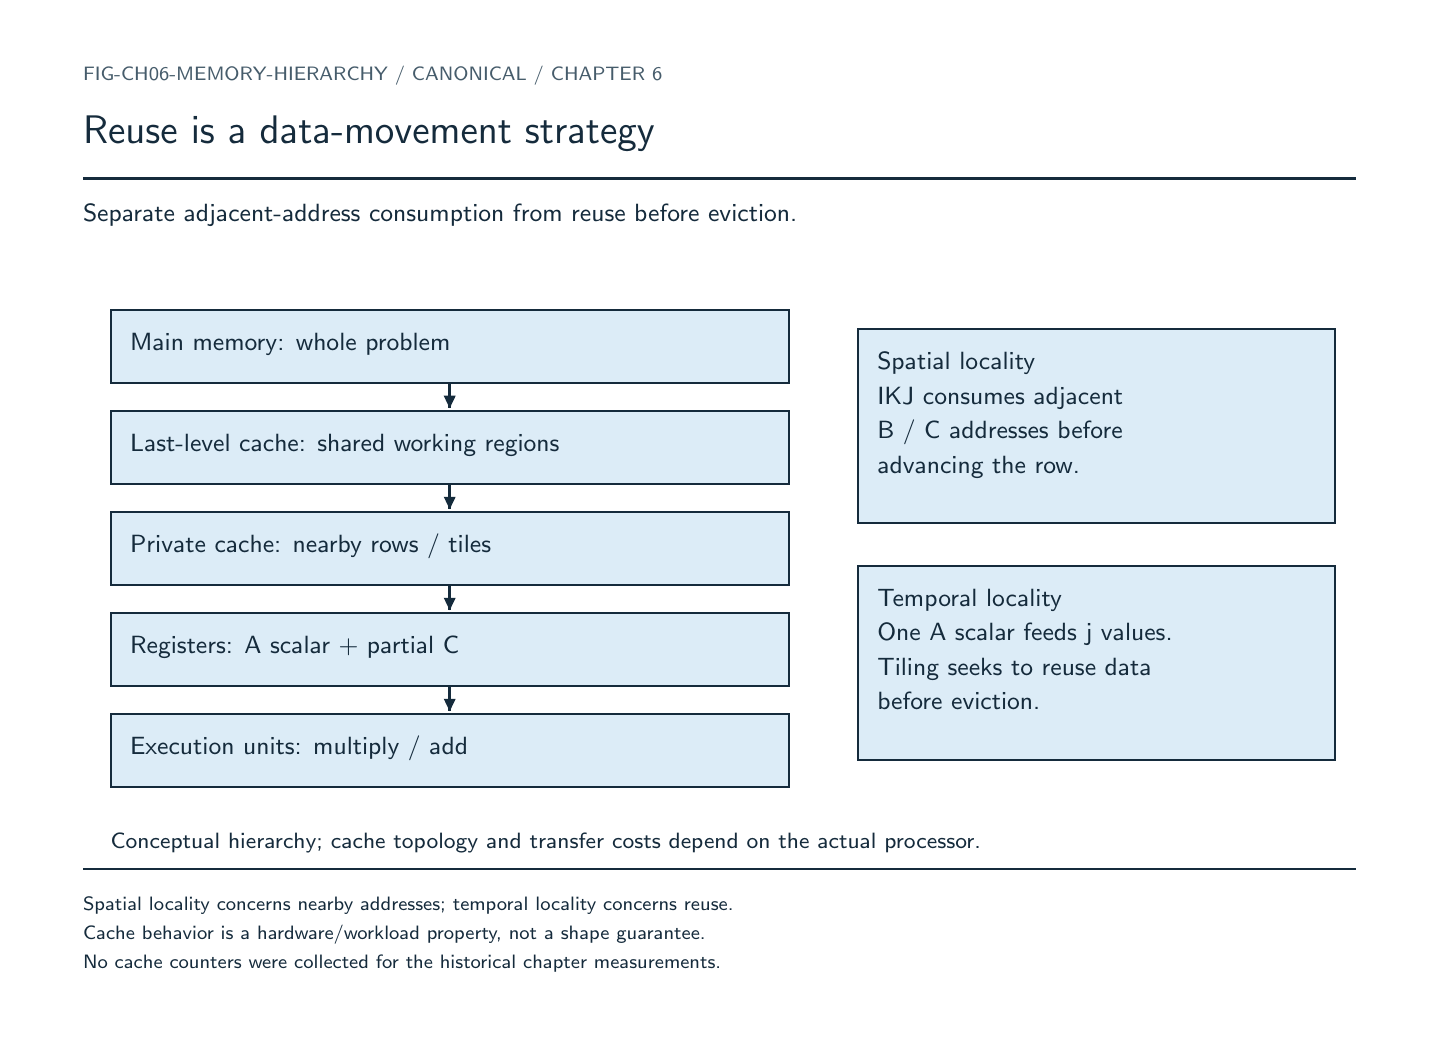
\begin{tikzpicture}[x=.5pt,y=-.5pt]
\path[use as bounding box] (0,0) rectangle (1000,720);
\path[fill=white,draw=none,line width=0.5pt] (0.0,0.0) rectangle (1000.0,720.0);
\node[inner sep=0pt,outer sep=0pt,anchor=base west,text={rgb,255:red,70;green,92;blue,107},font=\sffamily\fontsize{7.0}{8.4}\selectfont] at (40,38) {FIG-CH06-MEMORY-HIERARCHY  /  CANONICAL / CHAPTER 6};
\node[inner sep=0pt,outer sep=0pt,anchor=base west,text={rgb,255:red,21;green,43;blue,60},font=\sffamily\fontsize{15.0}{18.0}\selectfont] at (40,84) {Reuse is a data-movement strategy};
\draw[fill=none,draw={rgb,255:red,21;green,43;blue,60},line width=0.75pt] (40,109) -- (960,109);
\node[inner sep=0pt,outer sep=0pt,anchor=base west,text={rgb,255:red,21;green,43;blue,60},font=\sffamily\fontsize{9.5}{11.4}\selectfont] at (40,140) {Separate adjacent-address consumption from reuse before eviction.};
\path[fill={rgb,255:red,220;green,236;blue,247},draw={rgb,255:red,21;green,43;blue,60},line width=0.7pt] (60.0,204.0) rectangle (550.0,257.0);
\node[inner sep=0pt,outer sep=0pt,anchor=base west,text={rgb,255:red,21;green,43;blue,60},font=\sffamily\fontsize{9.0}{10.799999999999999}\selectfont] at (74,233) {Main memory: whole problem};
\node[inner sep=0pt,outer sep=0pt,anchor=base west,text={rgb,255:red,21;green,43;blue,60},font=\sffamily\fontsize{9.0}{10.799999999999999}\selectfont] at (74,258) {};
\draw[fill=none,draw={rgb,255:red,21;green,43;blue,60},line width=1.25pt] (305,257) -- (305,275);
\path[fill={rgb,255:red,21;green,43;blue,60},draw=none,line width=0.5pt] (305.00,275.00) -- (300.65,266.00) -- (309.35,266.00) -- cycle;
\path[fill={rgb,255:red,220;green,236;blue,247},draw={rgb,255:red,21;green,43;blue,60},line width=0.7pt] (60.0,277.0) rectangle (550.0,330.0);
\node[inner sep=0pt,outer sep=0pt,anchor=base west,text={rgb,255:red,21;green,43;blue,60},font=\sffamily\fontsize{9.0}{10.799999999999999}\selectfont] at (74,306) {Last-level cache: shared working regions};
\node[inner sep=0pt,outer sep=0pt,anchor=base west,text={rgb,255:red,21;green,43;blue,60},font=\sffamily\fontsize{9.0}{10.799999999999999}\selectfont] at (74,331) {};
\draw[fill=none,draw={rgb,255:red,21;green,43;blue,60},line width=1.25pt] (305,330) -- (305,348);
\path[fill={rgb,255:red,21;green,43;blue,60},draw=none,line width=0.5pt] (305.00,348.00) -- (300.65,339.00) -- (309.35,339.00) -- cycle;
\path[fill={rgb,255:red,220;green,236;blue,247},draw={rgb,255:red,21;green,43;blue,60},line width=0.7pt] (60.0,350.0) rectangle (550.0,403.0);
\node[inner sep=0pt,outer sep=0pt,anchor=base west,text={rgb,255:red,21;green,43;blue,60},font=\sffamily\fontsize{9.0}{10.799999999999999}\selectfont] at (74,379) {Private cache: nearby rows / tiles};
\node[inner sep=0pt,outer sep=0pt,anchor=base west,text={rgb,255:red,21;green,43;blue,60},font=\sffamily\fontsize{9.0}{10.799999999999999}\selectfont] at (74,404) {};
\draw[fill=none,draw={rgb,255:red,21;green,43;blue,60},line width=1.25pt] (305,403) -- (305,421);
\path[fill={rgb,255:red,21;green,43;blue,60},draw=none,line width=0.5pt] (305.00,421.00) -- (300.65,412.00) -- (309.35,412.00) -- cycle;
\path[fill={rgb,255:red,220;green,236;blue,247},draw={rgb,255:red,21;green,43;blue,60},line width=0.7pt] (60.0,423.0) rectangle (550.0,476.0);
\node[inner sep=0pt,outer sep=0pt,anchor=base west,text={rgb,255:red,21;green,43;blue,60},font=\sffamily\fontsize{9.0}{10.799999999999999}\selectfont] at (74,452) {Registers: A scalar + partial C};
\node[inner sep=0pt,outer sep=0pt,anchor=base west,text={rgb,255:red,21;green,43;blue,60},font=\sffamily\fontsize{9.0}{10.799999999999999}\selectfont] at (74,477) {};
\draw[fill=none,draw={rgb,255:red,21;green,43;blue,60},line width=1.25pt] (305,476) -- (305,494);
\path[fill={rgb,255:red,21;green,43;blue,60},draw=none,line width=0.5pt] (305.00,494.00) -- (300.65,485.00) -- (309.35,485.00) -- cycle;
\path[fill={rgb,255:red,220;green,236;blue,247},draw={rgb,255:red,21;green,43;blue,60},line width=0.7pt] (60.0,496.0) rectangle (550.0,549.0);
\node[inner sep=0pt,outer sep=0pt,anchor=base west,text={rgb,255:red,21;green,43;blue,60},font=\sffamily\fontsize{9.0}{10.799999999999999}\selectfont] at (74,525) {Execution units: multiply / add};
\node[inner sep=0pt,outer sep=0pt,anchor=base west,text={rgb,255:red,21;green,43;blue,60},font=\sffamily\fontsize{9.0}{10.799999999999999}\selectfont] at (74,550) {};
\path[fill={rgb,255:red,220;green,236;blue,247},draw={rgb,255:red,21;green,43;blue,60},line width=0.7pt] (600.0,218.0) rectangle (945.0,358.0);
\node[inner sep=0pt,outer sep=0pt,anchor=base west,text={rgb,255:red,21;green,43;blue,60},font=\sffamily\fontsize{9.0}{10.799999999999999}\selectfont] at (614,247) {Spatial locality};
\node[inner sep=0pt,outer sep=0pt,anchor=base west,text={rgb,255:red,21;green,43;blue,60},font=\sffamily\fontsize{9.0}{10.799999999999999}\selectfont] at (614,272) {IKJ consumes adjacent};
\node[inner sep=0pt,outer sep=0pt,anchor=base west,text={rgb,255:red,21;green,43;blue,60},font=\sffamily\fontsize{9.0}{10.799999999999999}\selectfont] at (614,297) {B / C addresses before};
\node[inner sep=0pt,outer sep=0pt,anchor=base west,text={rgb,255:red,21;green,43;blue,60},font=\sffamily\fontsize{9.0}{10.799999999999999}\selectfont] at (614,322) {advancing the row.};
\path[fill={rgb,255:red,220;green,236;blue,247},draw={rgb,255:red,21;green,43;blue,60},line width=0.7pt] (600.0,389.0) rectangle (945.0,529.0);
\node[inner sep=0pt,outer sep=0pt,anchor=base west,text={rgb,255:red,21;green,43;blue,60},font=\sffamily\fontsize{9.0}{10.799999999999999}\selectfont] at (614,418) {Temporal locality};
\node[inner sep=0pt,outer sep=0pt,anchor=base west,text={rgb,255:red,21;green,43;blue,60},font=\sffamily\fontsize{9.0}{10.799999999999999}\selectfont] at (614,443) {One A scalar feeds j values.};
\node[inner sep=0pt,outer sep=0pt,anchor=base west,text={rgb,255:red,21;green,43;blue,60},font=\sffamily\fontsize{9.0}{10.799999999999999}\selectfont] at (614,468) {Tiling seeks to reuse data};
\node[inner sep=0pt,outer sep=0pt,anchor=base west,text={rgb,255:red,21;green,43;blue,60},font=\sffamily\fontsize{9.0}{10.799999999999999}\selectfont] at (614,493) {before eviction.};
\node[inner sep=0pt,outer sep=0pt,anchor=base west,text={rgb,255:red,21;green,43;blue,60},font=\sffamily\fontsize{8.0}{9.6}\selectfont] at (60,593) {Conceptual hierarchy; cache topology and transfer costs depend on the actual processor.};
\draw[fill=none,draw={rgb,255:red,21;green,43;blue,60},line width=0.75pt] (40,608) -- (960,608);
\node[inner sep=0pt,outer sep=0pt,anchor=base west,text={rgb,255:red,21;green,43;blue,60},font=\sffamily\fontsize{7.5}{9.0}\selectfont] at (40,638) {Spatial locality concerns nearby addresses; temporal locality concerns reuse.};
\node[inner sep=0pt,outer sep=0pt,anchor=base west,text={rgb,255:red,21;green,43;blue,60},font=\sffamily\fontsize{7.5}{9.0}\selectfont] at (40,659) {Cache behavior is a hardware/workload property, not a shape guarantee.};
\node[inner sep=0pt,outer sep=0pt,anchor=base west,text={rgb,255:red,21;green,43;blue,60},font=\sffamily\fontsize{7.5}{9.0}\selectfont] at (40,680) {No cache counters were collected for the historical chapter measurements.};
\end{tikzpicture}
